% !TeX spellcheck = en_US
\documentclass[11pt, fleqn]{article}
%\usepackage{siunitx}
\usepackage{texfiles/SpeedyGonzales}
\usepackage{texfiles/MediocreMike}
\title{Logbook for 02466}
\author{Oskar Eiler Wiese Christensen, s183917@student.dtu.dk \\ Anders Henriksen, s183904@student.dtu.dk}

\begin{document}
	\maketitle
	
\section*{Project Meetings}

\subsection*{Week 1: 5.2.20 - 11.2.20}
We had no project meeting this week, as our group had not yet been created.

\subsection*{Week 2: 12.2.20 - 18.2.20}
\textbf{Questions:} At this point, there are no questions, as we had not started work on the project. \\
\textbf{Reading:} For the end of next week, we will attempt to read the central article to this project, "equality of opportunity in supervised learning", without necessarily going too much into the details. \\
\textbf{Implementation:} We will start implementing the neural network immediately, as this will be the foundation for the rest of the project.

\subsection*{Week 3: 19.2.20 - 25.2.20}


\subsection*{Week 4: 26.2.20 - 3.3.20}


\subsection*{Week 5: 4.3.20 - 10.3.20}


\subsection*{Week 6: 11.3.20 - 17.3.20}


\subsection*{Week 7: 18.3.20 - 24.3.20}


\subsection*{Week 8: 25.3.20 - 31.3.20}


\subsection*{Week 9: 1.4.20 - 5.4.20}


\subsection*{Week 10: 15.4.20 - 21.4.20}


\subsection*{Week 11: 22.4.20 - 28.4.20}


\subsection*{Week 12: 29.4.20 - 5.5.20}


\subsection*{Week 1: 6.5.20 - 12.5.20}


\subsection*{3-Week Period - Week 1: 4.6.20 - 10.6.20}


\subsection*{3-Week Period - Week 2: 11.6.20 - 17.6.20}


\subsection*{3-Week Period - Week 3: 18.6.20 - 24.6.20}



\section*{Supervisor Meetings}

\subsection*{Week 1: 5.2.20 - 11.2.20}
We had no supervisor meeting this week, as the project had not started yet.

\subsection*{Week 2: 12.2.20 - 18.2.20}
In this meeting, we set the foundation for how the following supervisor meetings will proceed. Our meeting will be at 13:00 every wednesday and the other group that has the same topic will have their meeting at 14:00. Every second week for the first part of the project process, our meetings will be combined, so we can learn from each other's mistakes and get common issues sorted out. \\
We will start the work on the research questions after this meeting and will be focusing on questions with concrete success criteria and a clearly defined scope. We were also urged to consider implementing multiple classification and bias correction algorithms. For next week, we will have outlined some research questions to go through.

\subsection*{Week 3: 19.2.20 - 25.2.20}


\subsection*{Week 4: 26.2.20 - 3.3.20}


\subsection*{Week 5: 4.3.20 - 10.3.20}


\subsection*{Week 6: 11.3.20 - 17.3.20}


\subsection*{Week 7: 18.3.20 - 24.3.20}


\subsection*{Week 8: 25.3.20 - 31.3.20}


\subsection*{Week 9: 1.4.20 - 5.4.20}


\subsection*{Week 10: 15.4.20 - 21.4.20}


\subsection*{Week 11: 22.4.20 - 28.4.20}


\subsection*{Week 12: 29.4.20 - 5.5.20}


\subsection*{Week 1: 6.5.20 - 12.5.20}


\subsection*{3-Week Period - Week 1: 4.6.20 - 10.6.20}


\subsection*{3-Week Period - Week 2: 11.6.20 - 17.6.20}


\subsection*{3-Week Period - Week 3: 18.6.20 - 24.6.20}


		
\newpage
\newpage
\section*{Project Meetings}
	
	%Questions \\
	%Reading, who and what \\
	%Implementation, who and what \\
	%Results, who and what \\
	%Decisions, who and what, what do you do alone, what do you do together
	
	\textbf{Week 08:}  19.02.2020 \\\\
	\noindent
	Hvilke bias eksisterer i dataen? \\ 
	\begin{figure}[H]
		\centering
		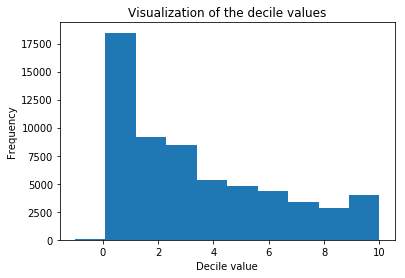
\includegraphics[width=0.3\linewidth]{billeder/decil.png}
	\end{figure}

	\begin{figure}[H]
		\centering
		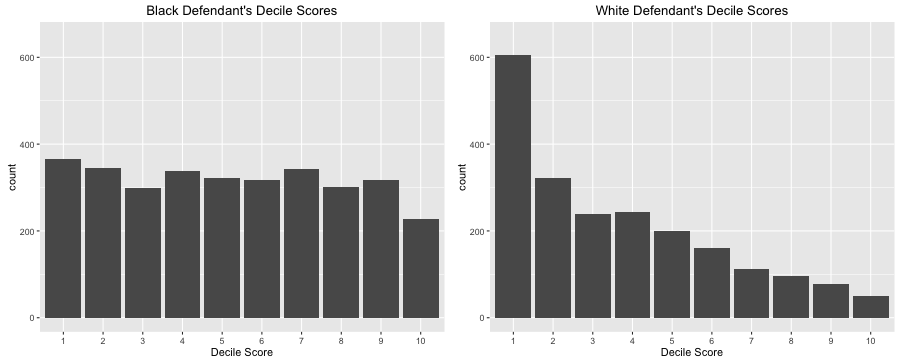
\includegraphics[width=0.7\linewidth]{billeder/black_white}
	\end{figure}
	\noindent
	There exists a recial bias in the dataset, which is indicated by the histograms above. 
	\\\\
	\textbf{Week 10:}  03.03.2020 \\\\
	\noindent
	Spørgsmål til næste møde: \\
	Hvordan skal dataen permuteres ? (Kun indenfor en kategorisk variabel eller hele datasættet) \newline 
	Kan man se bias ud fra confusion matrix?? \\ 
	Skal man vise, at der en statistisk forskel på de to confusion matricer? \\ \\
	\textbf{Noter} \\ 
	Lav nogle flere plots for at vise, om der er bias i selve data. Undersøg, hvor mange der får 1 i recidivism både af sorte og hvide.
	\newline
	Det ville være smart at finde noget statistisk signifikans. Man kan finde en p-værdi ved at bruge permutationstests.
	\newline
	Lav predictions med random forests.
	\newline
	Equal opportunity er godt resultatet, som vi ser fra vores data. Man kunne plotte equal opportunity som netværket bliver trænet.
	\newline
	Lav en slags baseline som logistisk regression for at se, om de begge er biased eller om de klarer sig lige godt.
	\newline
	Vi skal senest have midvejafleveringen klar d. 16, så Aasa kan læse det igennem.	
	\\\\	
	\textbf{Week 11:}  10.03.2020 \\\\
	\noindent
	Spørgsmål:
	\begin{itemize}
		\item  Hvordan skal vi lave feature selection for at se om de forskellige attributes påvirker modellen? Skal det stå som et afsnit i metoder?
		
		\item 4454, i forhold til at tage udgangspunkt i dataen, hvordan kan bias påvises vha. permutationstest. 
		
		\item Hvordan man helt præcist skal implementere Hardt et al. (post hoc correction)
		
		\item Hvordan skal vi finde bias i datasættet? 
		
		\item domain adaptation / transfer learning
		
		\item ting fra ICML / ECML , ICLR, Fair 
		
	\end{itemize}
	
	Skrive om feature selection i metode
	
	
\section*{Supervisor Meetings}
	
	\textbf{Week 07:}  12.02.2020 \\\\
	\noindent
%	Presentation of results since last meeting \\
	Meeting notes: \\ Fællesmøder samt personlige møde. (Hver anden uge er individuele). \\0. Vi får et datasæt (COMPASS) - ligger online \\
	1. Hvordan er dataen skæv? (Hvilke bias eksisterer i dataen) (Hvordan finder man helt præcist ud af det?) (Hvad betyder det at der er en bias?) \\
	2. Hvad gør skæv data ved min algoritme? (hvad betyder bias i en algoritme) (Hvordan kvantificeres/verificeres bias i algorimten?) \\
	3. Equality of Opportunity in Supervised Learning (forstå, implementer og valider) \\ 
	4. Etisk diskussion (Sune Filosof)
	\\\\\\\\
	\textbf{Week 08:}  19.02.2020 \\\\
	\noindent
	%	Presentation of results since last meeting \\
	Meeting notes: \\ Feature extraction
	\\\\
	Action points for next week: N/A
	\\\\\\\\
	\textbf{Week 09:}  26.02.2020 \\\\
	\noindent
	%	Presentation of results since last meeting \\
	Meeting notes: 
	\\\\
	Action points for next week
	\begin{itemize}
		\item  
	\end{itemize} 
		
	
\end{document}
